% =====================================================================
% EDITED EXCERPT — two-page progress note + thesis Sections 1–18
%
% The body pages (3–30) are Sections 1–18 of the working thesis, taken
% directly from the thesis build so the excerpt can never drift from
% the source it claims to sample.
%
% Build order, from the repository root:
%   python3 thesis/code/build.py thesis          # or: cd thesis && latexmk -pdf thesis-draft.tex
%   cd progress-report && latexmk -pdf edited-excerpt-30-pages.tex
% =====================================================================
\documentclass[11pt]{article}
\usepackage[letterpaper,margin=0.85in,top=0.75in,bottom=0.9in]{geometry}
\usepackage[T1]{fontenc}
\usepackage[scaled=0.95]{helvet}
\renewcommand{\familydefault}{\sfdefault}
\usepackage{xcolor}
\usepackage{graphicx}
\usepackage{pdfpages}
\usepackage[most]{tcolorbox}
\usepackage{enumitem}
\usepackage{fancyhdr}
\usepackage[colorlinks=true,linkcolor=navy,urlcolor=navy]{hyperref}

\hypersetup{
  pdftitle={Let the Machine Reveal Itself --- Thesis Progress Excerpt},
  pdfauthor={Jony (TUNEM)},
  pdfsubject={Two-page progress note plus thesis Sections 1--18},
  pdfkeywords={tokamak, fusion, thesis, progress report, TUNEM}}

% ---- house palette (shared with the illustrated guide and prospectus)
\definecolor{navy}{HTML}{1B3A5C}
\definecolor{gold}{HTML}{D4A028}
\definecolor{teal}{HTML}{1F7A8C}
\definecolor{cream}{HTML}{FFF8E7}
\definecolor{mist}{HTML}{EEF3F7}
\definecolor{ink}{HTML}{222222}
\definecolor{mute}{HTML}{666666}

\setlength{\parindent}{0pt}
\setlength{\parskip}{6pt}
\color{ink}

% ---- footer
\pagestyle{fancy}
\fancyhf{}
\renewcommand{\headrulewidth}{0pt}
\fancyfoot[L]{\footnotesize\color{mute}TUNEM thesis progress excerpt}
\fancyfoot[R]{\footnotesize\color{mute}\thepage}

% ---- building blocks
\newcommand{\kicker}[1]{\noindent{\footnotesize\bfseries\color{gold}\MakeUppercase{#1}}\par\vspace{4pt}}
\newcommand{\bigtitle}[1]{{\fontsize{26}{30}\selectfont\bfseries\color{white}#1\par}}
\newcommand{\subtitle}[1]{{\normalsize\color{white}#1}\par}
\newcommand{\heading}[1]{\vspace{10pt}{\large\bfseries\color{navy}#1}\par\vspace{2pt}}

\newtcolorbox{goldbox}[1]{enhanced, colback=cream, colframe=gold, boxrule=0.8pt,
  arc=3pt, left=8pt, right=8pt, top=6pt, bottom=6pt, fonttitle=\bfseries,
  coltitle=navy, title=#1, attach title to upper={\par\vspace{2pt}}, before skip=8pt, after skip=8pt}
\newtcolorbox{mapbox}[1]{enhanced, colback=mist, colframe=mist, boxrule=0pt,
  arc=3pt, left=8pt, right=8pt, top=6pt, bottom=6pt, fonttitle=\bfseries,
  coltitle=teal, title=#1, attach title to upper={\par\vspace{2pt}}, before skip=6pt, after skip=6pt}

\setlist[itemize]{label=\textcolor{teal}{\textbullet}, leftmargin=1.4em, itemsep=2pt, topsep=3pt}

% Full-width navy banner with gold rule beneath it
\newcommand{\banner}[3]{%
  \begin{tikzpicture}[remember picture, overlay]
    \fill[navy] (current page.north west) rectangle ([yshift=-2.05in]current page.north east);
    \fill[gold] ([yshift=-2.05in]current page.north west) rectangle ([yshift=-2.12in]current page.north east);
  \end{tikzpicture}%
  \vspace*{-0.15in}
  \kicker{#1}
  \bigtitle{#2}
  \vspace{4pt}
  \subtitle{#3}
  \vspace{1.15in}
}

\begin{document}

% ======================================================= PAGE 1
\banner{Thesis progress report \,|\, September 2026}{Let the Machine Reveal Itself}{A first-principles construction of the tokamak --- Sections 1--18}

\heading{Purpose of this excerpt}
This packet presents the opening act of a larger working thesis. It does not begin with a finished tokamak.
It starts with controlled D--T fusion and allows each failure of the simplest attempted design to force the
next field, component, or parameter into existence.

\begin{goldbox}{The governing philosophy}
Minimum assumptions, not minimum physics. Every load-bearing statement is derived, identified as a model,
or tied to a source. The machine gradually reveals itself rather than being presented as an unexplained object.
\end{goldbox}

\heading{What the 28-page excerpt contains}
\begin{itemize}
  \item Fusion temperature, plasma formation, and magnetic steering from the Lorentz force.
  \item The failure of a straight magnetic corridor and the geometric necessity of a torus.
  \item Toroidal drift, plasma current, the poloidal field, safety factor, and equilibrium control.
  \item Heating, elongation, current-profile control, and the first conditional performance scaling.
  \item A Section 18 ledger stating exactly what has and has not yet been derived.
\end{itemize}

\vfill
{\footnotesize\color{mute}
The pages that follow are Sections 1--18 of the working thesis draft, reproduced from the current thesis build.
The separate illustrated guide maps the full argument (\S\S1--127); the full draft contains the longer derivations.}

\clearpage

% ======================================================= PAGE 2
\kicker{Progress and discussion map}
{\fontsize{22}{26}\selectfont\bfseries\color{navy}Where the full draft is going\par}
\vspace{6pt}

The complete working PDF is substantially longer than this packet. The excerpt was chosen because Section 18
forms a natural first-act conclusion and remains elementary enough for careful verification in one or two days.

\begin{mapbox}{1. Derive the machine and its vocabulary}
Sections 1--50 derive the fields, geometry, current, shaping, confinement quantities, nuclear island, and
magnet radial build.
\end{mapbox}

\begin{mapbox}{2. Reconstruct the Freidberg design argument}
Sections 51--101 rebuild the 2015 conventional reference, expose its assumptions, test its constraints, and
compare its proposed remedies.
\end{mapbox}

\begin{mapbox}{3. Test the low-aspect-ratio branch}
Sections 102--111 show why lower aspect ratio changes the kink and bootstrap mechanisms. The published
candidate closes the kink test; bootstrap closure remains conditional on independently affordable current drive.
\end{mapbox}

\begin{mapbox}{4. Confront the centre-stack bargain}
Sections 112--127 derive the separate radial, current-density, stress, shielding, startup, and HTS obligations
created by the low-$A$ geometry. They establish the conventional centre-stack ledger; connecting that ledger to
solenoid-light merging-compression startup is the six-week study proposed in the accompanying prospectus.
\end{mapbox}

\heading{Questions for discussion}
\begin{itemize}
  \item Is the derive-before-design structure appropriate for the intended reader?
  \item Which approximations should receive a fuller derivation, a stronger source, or earlier qualification?
  \item Would the adjacent six-week centre-stack/startup feasibility study be useful to the group?
  \item Which recent papers, models, or current group problems should define the next research step?
\end{itemize}

\begin{goldbox}{Academic objective}
Complete the thesis and earn one useful joint technical paper, with the hope of sustaining collaboration
during a future physics PhD.
\end{goldbox}

\clearpage

% ======================================================= PAGES 3–30: thesis Sections 1–18
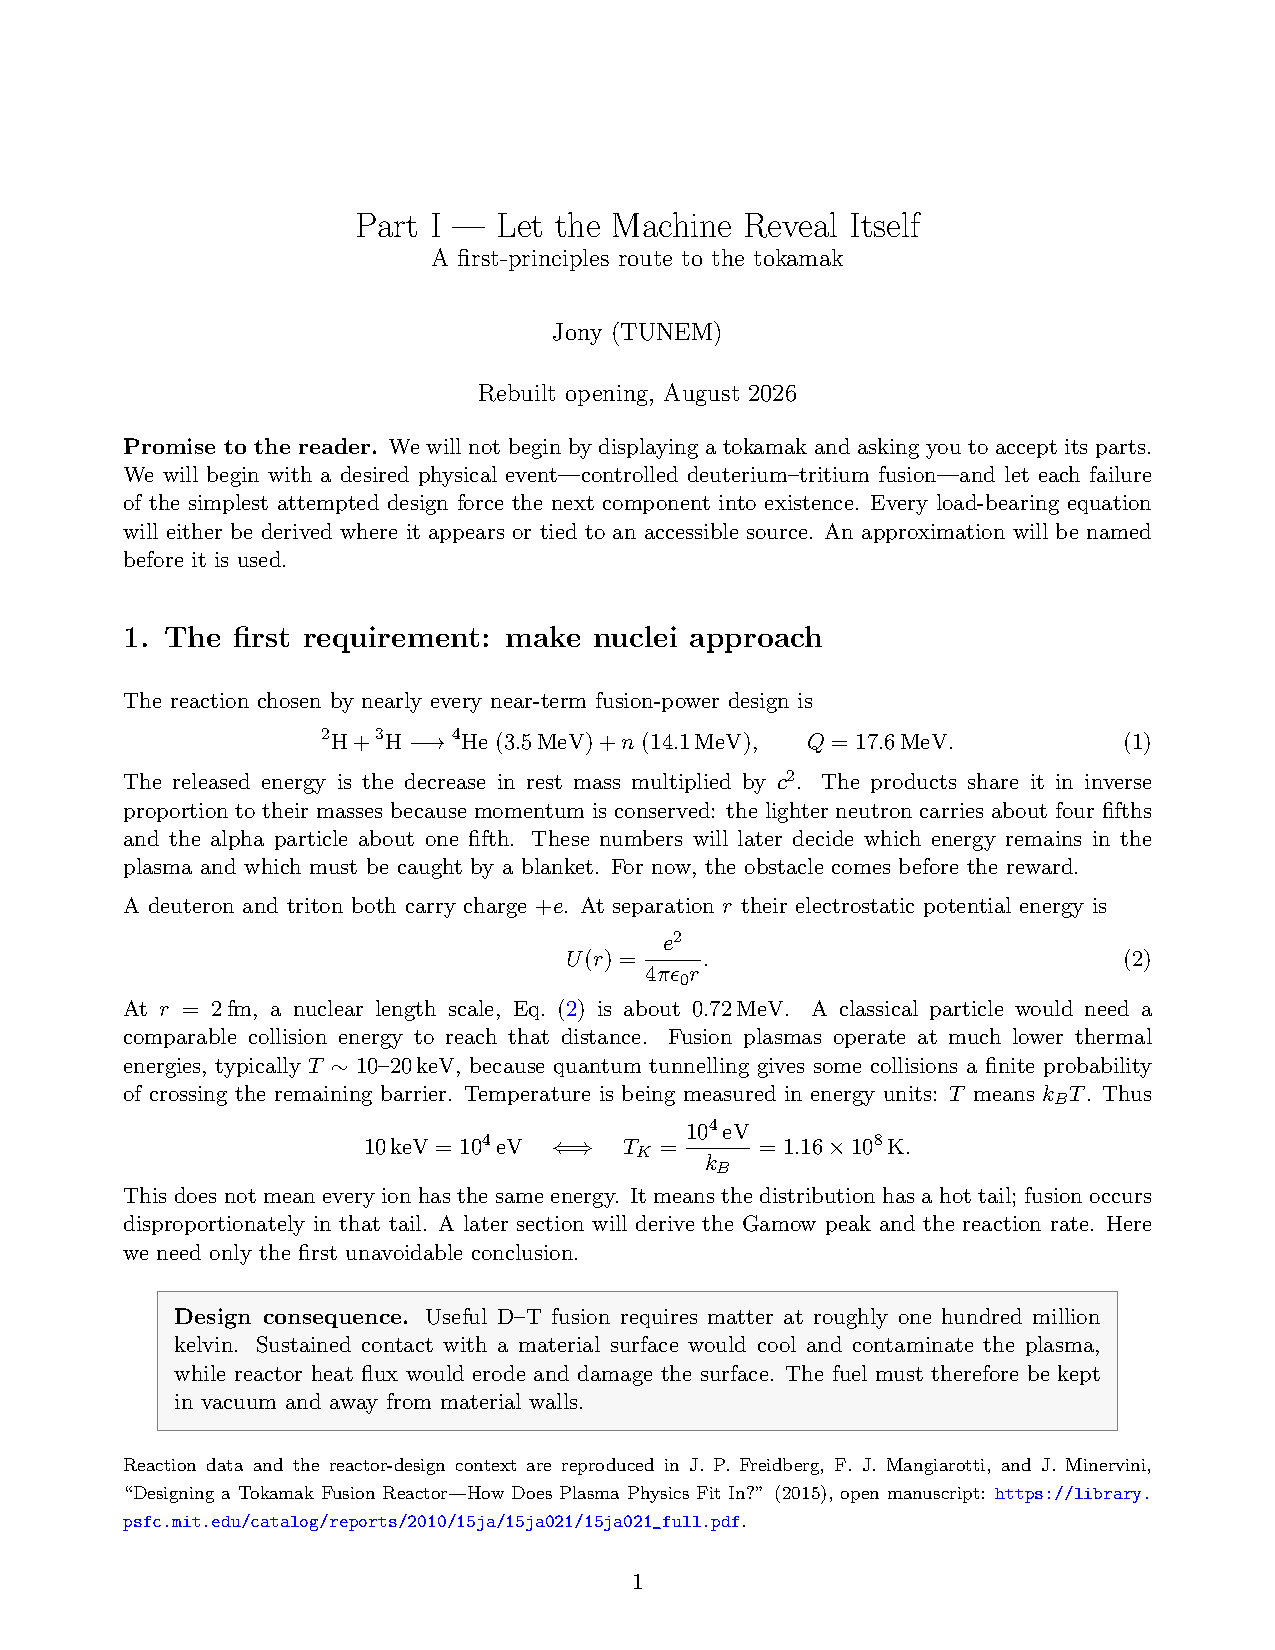
\includepdf[pages=1-28, pagecommand={\thispagestyle{empty}}]{../thesis/thesis-draft.pdf}

\end{document}
